%! Author = leona
%! Date = 09/02/24
% !TeX root = ../thesis-main.tex

\chapter{Validation}
\label{chap:validation}

The validation for this thesis' work has been done on multiple axes, which will be described in this chapter.

\section{Unit Testing}
The first layer of testing is the ``Unit Testing''. In computer science, this term refers to the act of analyzing and scrutinizing the smallest units of software possible.
This thesis adheres to Rust's unit testing practices: each public module that is part of the library has a corresponding and private testing module, annotated with the
conditional compilation macro ``\#[cfg(test)]'', denoting this is a module that is only compiled when the test suite is run.\\
Inside this module, it is possible to write test functions by annotating them with the ``\#[test]'' attribute. These functions can then be run with the ``cargo test'' command.\\
As such, each module in the RuFi library crates has a corresponding testing module containing unit test functions for them. For example, the listing \ref{lst:unit_test} shows the unit tests for the
vm\_status module.

\lstinputlisting[language=Rust, label={lst:unit_test}]{listings/unit_test.rs}

\section{Integration Testing}
Unit testing is a crucial practice in the development of software artifacts, but testing each component in isolation is not sufficient to analyze every aspect of the software produced.
Another important practice is the act of testing some or many components together, to ensure that their behavior when interacting is the one expected, which is called ``Integration Testing''.
Again, this thesis adheres to Rust's integration testing practices: each library crate has a corresponding ``tests'' directory, where integration tests are written. These tests are run with the ``cargo test'' command, just like their unit counterpart.\\
Inside the tests directory, it is possible to create various source files for testing. Each file is isolated from one another and is external to the library since it is compiled as an individual crate: this means that the
code inside these test files utilizes the library via its public API just like any other client code.\\
The listing \ref{lst:integration_test} shows an example of an integration test for the RuFi library that combines features coming from the RoundVM, Export and Language.

\lstinputlisting[language=Rust, label={lst:integration_test}]{listings/integration_test.rs}

\section{User Acceptance Testing}
A third axes along which the thesis' work has been validated is the ``User Acceptance Testing'', which refers to the practice of testing the software in a real-world scenario.
In particular, this involved the development of a demo project that exploits the RuFi framework to execute a gradient aggregate program within a network of 5 devices, each one
represented by a process running on a machine. At an application level, the topology is linear, meaning each device $i$ is a neighbor of the devices $i+1$ and $i-1$, excluding 1 and 5
which are the extremes of the topology. At a deployment level, there are four processes each one simulating a device run on a Desktop PC, while the fifth runs on a Raspberry Pi 3.\\
Each process communicates with the others through the MQTT protocol via the public Mosquitto MQTT broker. A graphical representation of the network is shown in figure \ref{fig:network_topology}.

\begin{figure}[ht!]
    \centering
    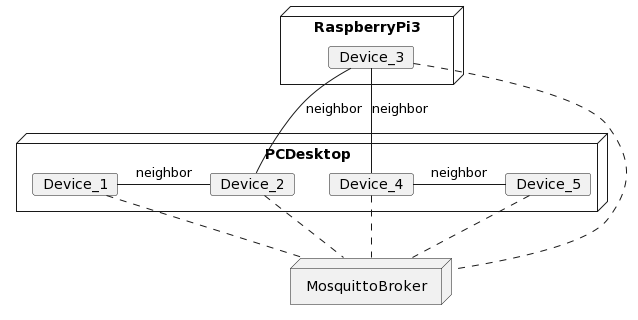
\includegraphics[width=0.8\textwidth]{figures/diagrams/img/deployment-demo.png}
    \caption{Network Topology}
    \label{fig:network_topology}
\end{figure}

\section{Memory Profiling}

\section{Quality Control}
